\subsection{Pumpenansteuerung}\label{subsec:Hardware_Pumpenansteuerung}

Die Pumpenansteuerung gemäss Kapitel \ref{subsec:Detailkonzept_Pumpenansteuerung} besteht lediglich aus einem Logic-FET, einer Diode und zwei Widerständen. Die Anforderungen an die Schaltung sind für den Verwendungszweck relativ gering. In Abbildung \ref{fig:Schaltverhalten_Pumpen} kann der Schaltmoment begutachtet werden. 

\begin{figure}[h!]
	\centering
	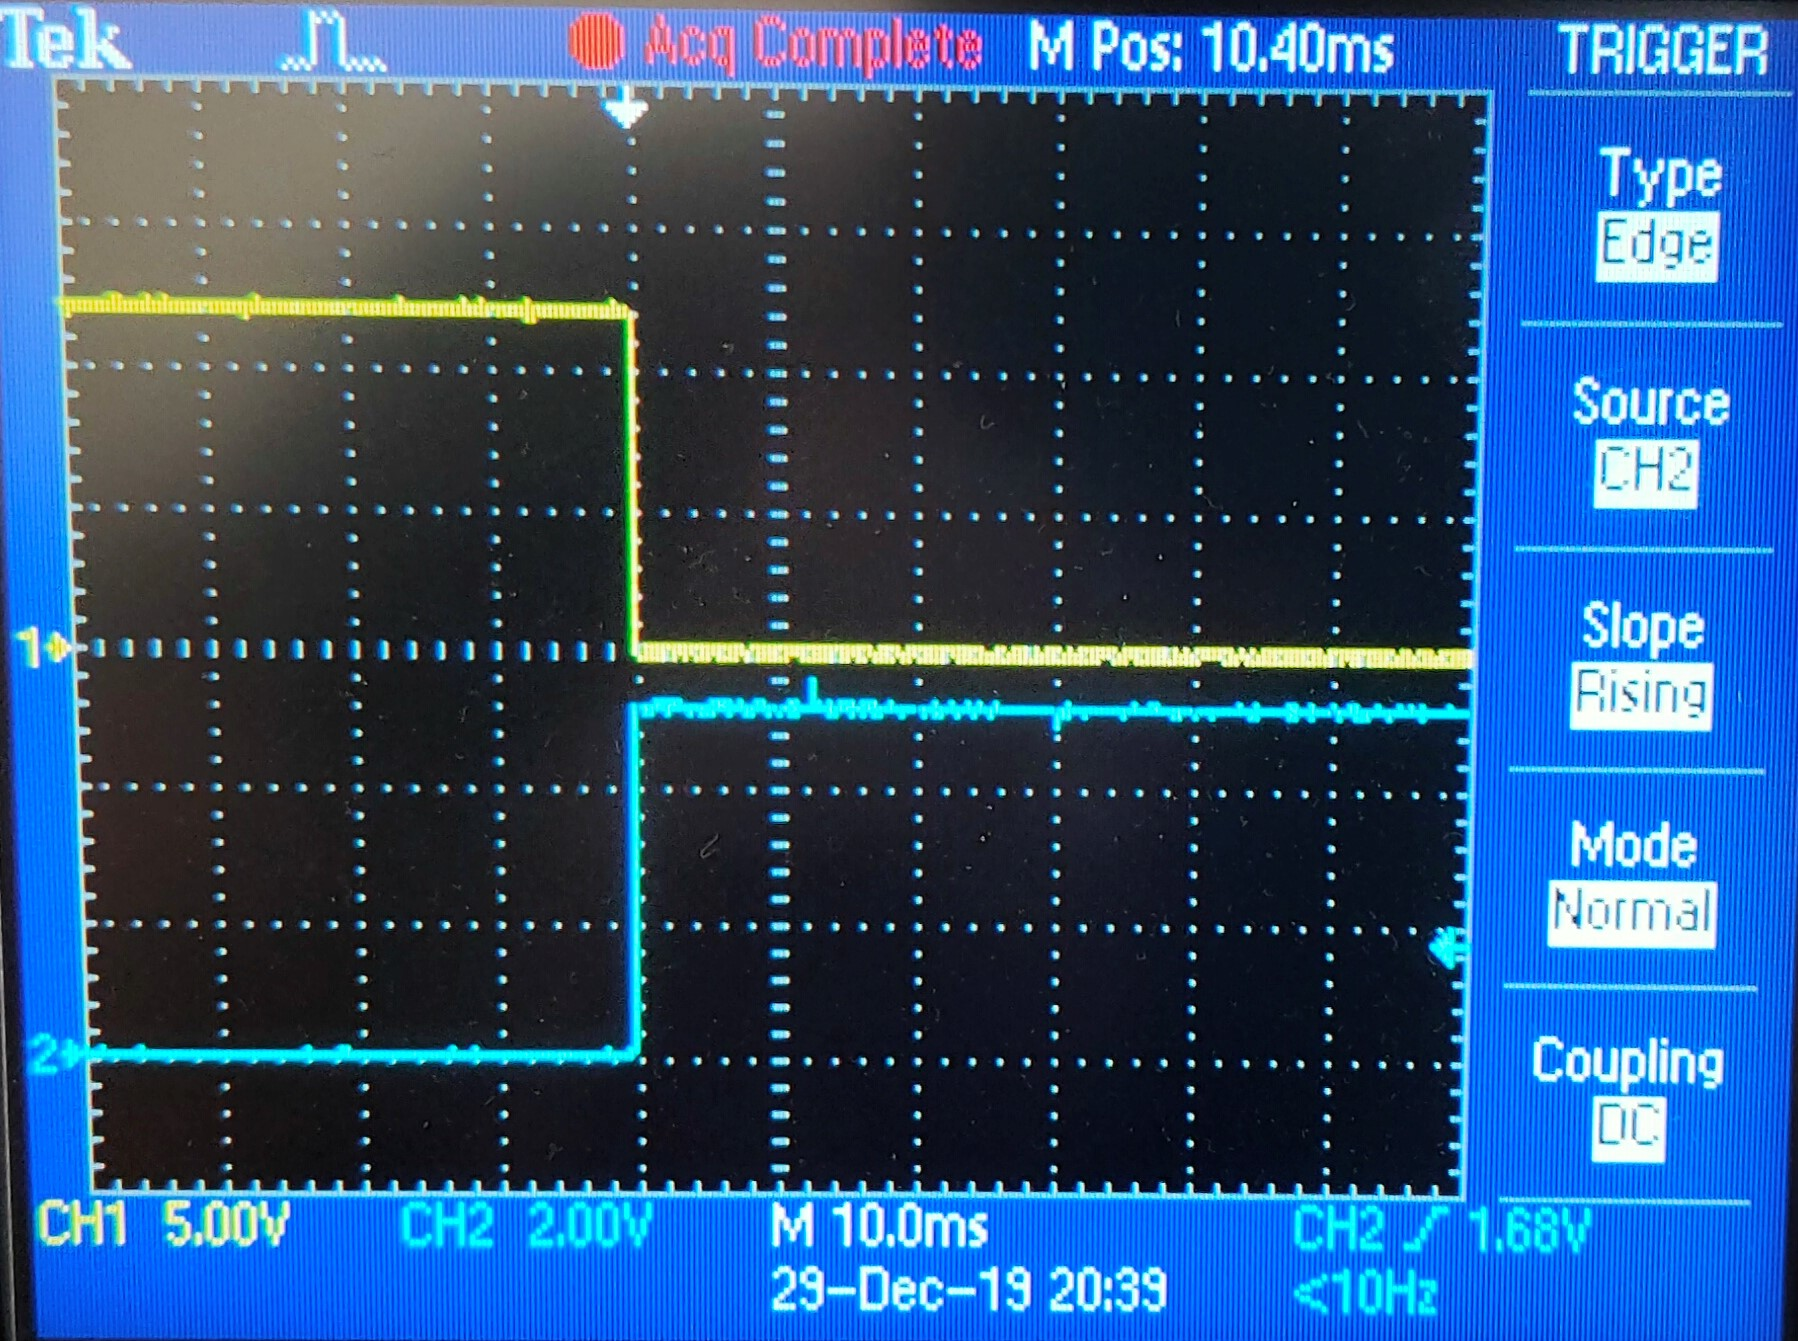
\includegraphics[width=0.8\textwidth]{graphics/PumpenMessung.jpg}
	\caption{Messung der Schalteigenschaft der Pumpenansteuerung} 
	\label{fig:Schaltverhalten_Pumpen}
\end{figure}

Folgende Spannungen und Ströme sind in Abbildung \ref{fig:Schaltverhalten_Pumpen} zu sehen: 

\begin{itemize}
	\item 1 Speisespannung am Drain
	\item 2 Gatespannung 
\end{itemize}

Es wird Wert darauf gelegt, dass der Logic-FET bei erfolgter Ansteuerung komplett durchsteuert. Die Anstiegszeit der Schaltflanke ist für diesen Zweck irrelevant. Daher wird diese auch nicht weiter detailliert verfolgt. 

\subsection{Durchflussmessgeräte}\label{subsec:Hardware_Durchflussmessgeraete}

Um zu sehen wie exakt mit den Durchflussmessgeräten gearbeitet werden kann, wurden einige Versuchsreihen durchgeführt. Dabei ist in einem ersten Schritt ein Programm in C erstellt worden, welches eine Pumpe über die in Kapitel \ref{subsec:Detailkonzept_Pumpenansteuerung} erwähnte Pumpenansteuerung ein- und ausschalten kann. Danach wurde ein Digitaleingang implementiert, welcher die erzeugten Pulse des Durchflussmessgerätes bei erfolgendem Durchfluss einlesen kann. Somit ist man nun in der Lage, durch das Zählen der Pulse, den Durchfluss zu bestimmen. 

Da vom Händler bei Aliexpress kein Datenblatt abgelegt wurde, wurde in einer ersten Phase ermittelt, wie viele Pulse bei einer gewünschten Menge von 250ml eingelesen werden. Dabei ergab sich ein Wert von 981 Pulsen bei 250ml. Danach wurde diese Füllmenge 10 Mal abgefüllt und die Ergebnisse miteinander verglichen. Es wurde dabei eine Toleranz von weniger als 0.5\% festgestellt. In einer Zweiten Messreihe wurden die 981 Pulse auf 3l hochgerechnet und dieser Wert ausgelesen. Dabei sollte beim Erreichen von 3924 Pulsen 3l Flüssigkeit abgefüllt sein. Bei diesem Test wurde eine Genauigkeit von 2.7\% festgestellt. 

All diese Versuche wurden vorgängig durchgeführt, bevor die eigentliche Evaluation starten sollte, um zu sehen wie gut alles arbeitet und ob die Toleranzen eingehalten werden können. Leider ist durch ein Missgeschick das vorhandene Durchflussmessgerät zerstört worden, wesshalb keine ausführliche Evaluation mit den dazugehörigen Messwerten durchgeführt werden konnte. Somit kann nur gesagt werden, dass die Messgeräte die erforderlichen Toleranzen einhalten, aber diese in Projekt 6 nochmals auf deren Genauigkeit geprüft werden müssen, sobald die neuen Messgeräte angekommen sind.